\section{Verification Design For Test}
\subsection{Warum testen?}$~$ \\
In der Fabrikation von elektronischen Systemen gibt es unzählige Fehlerquellen. Je früher ein Fehler erkennt werden kann, desto weniger teuer kommt er zu stehen. Eine Regel besagt, dass die Kosten mit jedem Produktionsschritt, bei welchem der Fehler nicht erkannt wurde, um den Faktor 10 ansteigen. Bei der Herstellung von digitalen Chips kann in der Regel mit einer Ausbeute von 95 bis 98\% gerechnet werden.

\subsection{Begriffe}
\begin{description}
  \item[Defect] Physikalische Fehlerquelle in integrierten Schaltungen
  \item[Fault] Messbare Fehlfunktion einer Schaltung aufgrund von einem/mehreren Fehler(n)
  \item[Quality] Mass für die exakte Erfüllung der Vorgaben (4 Bereiche: Design-, Herstellungs-, Auslieferungs- und Betriebsqualität)
  \item[Yield] Verhältnis von funktionierenden Teilen auf einem Wafer: $y_f = \frac{\#good\_circuits}{\#manufactured\_circuits}$
  \item[Defect level] Anteil an nicht-funktionierenden Chips, die unerkannt bleiben: $D_L = \frac{\#defective\_sold}{\#total\_sold} = 1 - y_f^{1-F_c}$
  \item[Fault coverage] Anteil an Fehlern die mit einem Set von Testvektoren erkannt werden können: $F_c = \frac{\#detectable\_Faults}{\#possible\_Fault}$
\end{description}


\subsection{Fehlermodelle}$~$ \\
Die nachfolgenden Fehlermodelle gibt es:
\begin{compactitem}
    \item \textbf{Stuck-At-0-Fault / Stuck-At-1-Fault}: Das entsprechende Signal wird auf einem Low-Pegel (Stuck-At-0-Fault) oder auf einem High-Pegel (Stuck-At-1-Fault) festgehalten und kann sich nicht ändern.
    \item \textbf{Bridging-Fault}: Bezeichnet einen Kurzschluss zwischen zwei Signalen. Ein Kurzschluss nach VDD oder VSS äussert sich wie ein Stuck-At-X-Fault. Ein Kurzschluss zwischen zwei Signalleitungen, verhält sich wie ein OR oder AND und kann im besten Fall funktional nachgewiesen werden.
    \item \textbf{Delay-Fault}: Dies sind eigentlich keine funktionalen Fehler, sondern Fehler in der Verzögerungszeit, hervorgerufen durch zu hohe Widerstandswerte der Verbindungen. Sie äussern sich letztlich jedoch funktional.
\end{compactitem}

\subsection{Fehlererkennung}
\subsubsection{Detektion von Stuck-At-X-Fault}
Um einen solchen Fehler zu detektieren, muss der entsprechende Knoten kontrollier- und beobachtbar sein. Kontrollierbar ist er dann, wenn er über ein externes Signal auf Low oder High gesetzt werden kann. Beobachtbar ist er dann, wenn sein Zustand von aussen überprüft werden kann.
\paragraph{Beispiel}$~$ \\
Anhand untenstehender Schaltung, wird nun eine Tabelle mit allen Testvektoren erstellt. In der Y-Spalte steht der Ausgangswert, wenn kein Fehler vorhanden ist. In den nachfolgenden Spalten, steht der Ausgangswert wenn der entsprechende Stuck-At-Fehler vorhanden ist.\ \\
\begin{minipage}{0.6\textwidth}
\begin{figure}[H]
    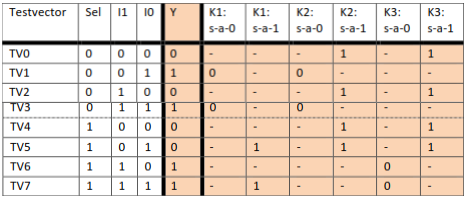
\includegraphics[width=1.0\textwidth]{images/stuckat_detektion_1.png}
\end{figure}
\end{minipage}
\hfill
\begin{minipage}{0.35\textwidth}
\begin{figure}[H]
    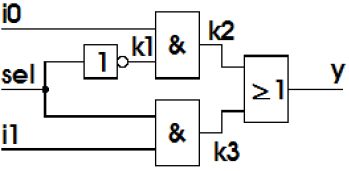
\includegraphics[width=1.0\textwidth]{images/stuckat_detektion_schaltung.png}
\end{figure}
\end{minipage} \\
Nun soll anhand der erstellten Tabelle, die Testvektorenanzahl auf ein Minimum beschränkt werden (Fault Collapsing). Mit den Testvektoren TV1, TV5 und TV7 kann somit jeder Fehler detektiert werden.
\begin{figure}[H]
    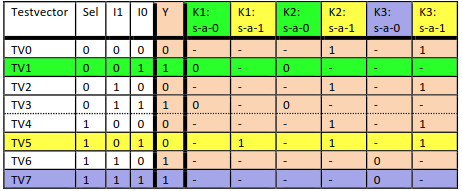
\includegraphics[width=0.6\textwidth]{images/stuckat_detektion_2.png}
\end{figure}

\subsubsection{Fehlerabdeckung (Fault coverage)}
Die Fehlerabdeckung kann folgendermassen berechnet werden: $\text{Fehlerabdeckung}=\frac{\text{Anzahl detektierter Fehler}}{\text{Abzahl möglicher Fehler}}*100\%$ Im Allgemeinen sollte darauf geachtet werden, dass eine Fehlerabdeckung von mindestens 95\% erreicht wird.

\subsubsection{Redundante Logik}
Sollte redundante Logik eingebaut sein (zur Verhinderung von Hazards), so kann die Funktion nicht ohne Zusatzaufwand getestet werden.
\paragraph{Beispiel}$~$ \\
Anhand von untenstehender Schaltung, wird die nachfolgende Tabelle erstellt. Dabei stellt sich heraus, dass ein Stuck-At-0-Fault am Knoten K4 nicht detektiert werden kann. Wenn aber die am Ausgang angeschlossene Logik darauf baut dass kein Hazard auftritt, kann dies zu einem Fehlverhalten führen.\\
\begin{minipage}{0.6\textwidth}
\begin{figure}[H]
    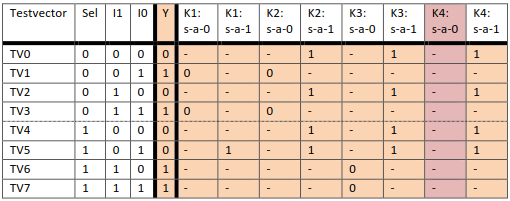
\includegraphics[width=1.0\textwidth]{images/stuckat_redundant_1.png}
\end{figure}
\end{minipage}
\hfill
\begin{minipage}{0.35\textwidth}
\begin{figure}[H]
    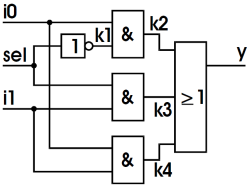
\includegraphics[width=1.0\textwidth]{images/stuckat_redundant_schaltung.png}
\end{figure}
\end{minipage}
\subsection{I\textsubscript{DDQ}-Test}$~$ \\
\begin{multicols}{2}
Beim I\textsubscript{DDQ}-Test wird die Ruhestromaufnahme der Schaltung gemessen. Dieser Ruhestrom ist im Normalfall vernachlässigbar klein. Entsteht jedoch bei einem Signalwert ein Kurzschluss, so ist dies über den Ruhestrom feststellbar. Wird bei einer Schaltung festgestellt, dass direkt nach dem Anlegen der Versorgungsspannung ein hoher Strom fliesst, kann auf nachfolgende Tests direkt verzichtet werden, was die Testzeit stark verkürzt.
\begin{figure}[H]
    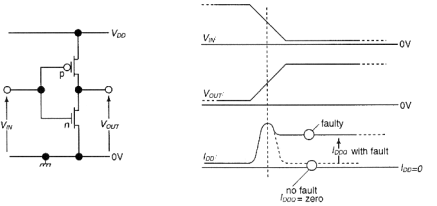
\includegraphics[width=0.5\textwidth]{images/iddq.png}
\end{figure}
\end{multicols}

\subsection{Scan Path}$~$ \\
Die Scan Path Methode adressiert das Problem, dass interne Knoten von aussen schlecht kontrollierbar und beobachtbar sind. Dazu wird vor jedes Flipflop ein 2:1 Multiplexer geschalten (Scan Flipflop), mit dessen Hilfe alle Flipflops zu einem riesigen Schieberegister zusammengeschaltet werden. \\
\begin{minipage}{0.25\textwidth}
\begin{figure}[H]
    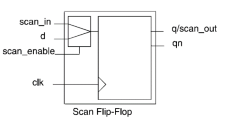
\includegraphics[width=1.0\textwidth]{images/scanflipflop.png}
\end{figure}
\end{minipage}
\hfill
\begin{minipage}{0.7\textwidth}
Die folgenden speziellen Signale sind nun vorhanden:
\begin{compactitem}
    \item \textit{scan\_enable}: Legt die Multiplexer Stellung fest.
    \item \textit{scan\_in}: Eingangssignal für das Schieberegister. Wird während dem Normalbetrieb nicht benötigt.
    \item \textit{scan\_out}: Ausgangssignal des Schieberegisters. Führt auf den \textit{scan\_in} Eingang des nächsten Flipflops.
\end{compactitem}
\end{minipage}

In einem ersten Schritt wird das ganze Schieberegister seriell befüllt. Damit können alle internen Eingänge kontrolliert werden. In einem zweiten Schritt wird das System für einen Taktzyklus in den Normalbetrieb versetzt. Im letzten Schritt wird das Schieberegister nun wieder seriell ausgelesen.

\subsubsection{Parallele Pfade}
Je mehr Flipflops sich in einem Design befinden, umso länger wird der Scan Pfad und somit auch die Testzeit. Durch die Verteilung der Flipflops auf mehrere Scan Pfade wird die Testdauer verkürzt. Es wird dabei versucht, die Scan Pfade möglichst auszubalancieren, damit es bei allen Pfaden gleich lange dauert um die Daten auszulesen oder zu schreiben.

\begin{multicols}{2}
    \subsubsection{Scan Path bei mehreren Taktdomänen}
    Sind in einem System unterschiedliche Taktdomänen vorhanden, so kommen Lock-Up Latches, an den Übergängen von einer Domäne zur anderen, zum Einsatz. Diese stellen sicher, dass keine laufzeitbedingten Fehler auftreten.

    \subsection{BIST (Built In Self Test)}$~$ \\
    Der Test von grossen programmierbaren Blöcken (z.B. RAM, ROM, PLA, ...) ist mit Scan Paths nur schwer möglich, da die Anzahl Testvektoren nicht wirklich reduziert werden kann, da auch wirklich jede Zelle überprüft werden muss. Aus diesem Grund wird jeder Makrozelle eine zusätzliche Logik zugeordnet, mit welcher diese einen Selbsttest durchführen kann. \ \\ \ \\
    \begin{figure}[H]
        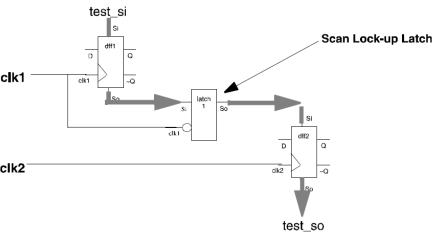
\includegraphics[width=0.5\textwidth]{images/scanpath_lookuplatch.png}
    \end{figure}
\end{multicols}

\subsubsection{Prinzip}
\begin{multicols}{2}
\begin{figure}[H]
    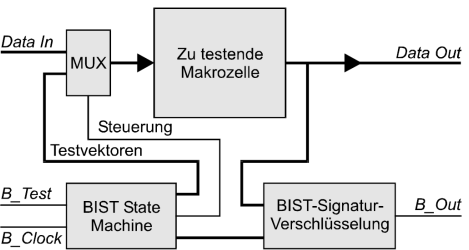
\includegraphics[width=0.5\textwidth]{images/prinzip_bist.png}
\end{figure}
Nebenstehend ist der prinzipielle Aufbau einer BIST-Zusatzlogik zu sehen. In den Eingangspfad der zu testenden Makrozelle ist ein 2:1-Multiplexer geschaltet. Über den Block BIST State Machine, der die Steuerlogik und einen Testmustergenerator enthält, wird dieser Multiplexer so geschaltet, dass entweder von aussen kommende Daten an die Makrozelle geführt werden (Normalbetrieb), oder solche vom Testmustergenerator (Testbetrieb). Die Ausgänge der Makrozelle werden neben der normalen Verdrahtung dem Block BIST-Signature-Verschlüsselung zugeführt. Dieser wertet die Testergebnisse aus und meldet sie nach aussen.
\end{multicols}

\subsection{BST (Boundary Scan Test)}$~$ \\
Die zunehmende Packungsdichte erschwert den Test von fertigen Baugruppen erheblich. Um die Anzahl erforderliche Prüfanschlüsse zu minimieren, wurde der BST entwickelt.

\begin{multicols}{2}
    \subsubsection{Konzept}
    Jeder Ein- und Ausgang eines Chips wird mittels einer BSC (Boundary Scan Cell) vom Kern der Schaltung abgetrennt. Alle diese BSCs sind wiederum zu einem grossen Schieberegister zusammengeschalten (BSR - Boundary Scan Register).

    \paragraph{Signale}$~$ \\
    Jeder Chip stellt nach Aussen die folgenden Signale zur Verfügung, resp. benötigt die folgenden Signale:
    \begin{compactitem}
        \item \textit{TDI}, \textit{TDO}: Test Data In / Test Data Out, werden auf der Leiterplatte zu einem Schieberegister verknüpft. Sprich jeder TDO führt auf den TDI des nächsten Chips.
        \item \textit{TCK}: Test Clock
        \item \textit{TMS}: Test Mode Select
        \item \textit{TRST*}: Optional, bringt den Chip in einen definierten Zustand
    \end{compactitem}

    \subsubsection{Realisierung auf dem Chip}
    Jeder Chip muss für BST die folgenden Elemente beinhalten:
    \begin{compactitem}
        \item \textbf{Bypass-Register}: Überbrückt dass BSR. So kann der entsprechende IC bei gewissen Test übersprungen werden. Dies verkürzt wiederum die Testdauer.
        \item \textbf{Device-ID-Register}: Enthält eine ID des Chips. Dieses Register kann während dem Test ausgelesen wertden um z.B. auf korrekte Bestückung zu prüfen.
        \item \textbf{TAP (Test Access Port)}: Schnittstelle nach Aussen
        \item \textbf{Instruction-Register}: Steuert die internen notwendigen Multiplexer Einstellungen.
    \end{compactitem}
    \begin{figure}[H]
        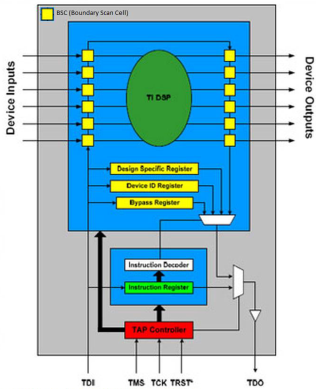
\includegraphics[width=0.5\textwidth]{images/bst_aufbau.png}
    \end{figure} \ \\ \ \\
\end{multicols}

\begin{multicols}{2}
    \subsubsection{TAP-Kontroller}
    Die Funktion des TAP-Kontrollers ist in nebenstehender Grafik dargestellt. In den Zustand \textit{Test-Logic-Reset} wird gewechselt wenn das \textit{TRST*}-Signal gesetzt wird oder indem das Signal \textit{TMS} während fünf Taktzyklen auf einem High-Pegel gehalten wird.

    \subsubsection{Instruktionen}
    \paragraph{Instruktions-Register}
    Das Instruktions-Register muss mindestens eine Länge von zwei Bit aufweisen um die verbindlichen Befehle dekodieren zu können. Das Register kann aber durchaus grösser sein, da viele Hersteller noch eigene Befehle implementieren. \\
    Wenn der TAP-Kontroller sich im Zustand \textit{Shift\_IR} befindet, wird die Instruktion seriell vom Eingang \textit{TDI} in das Instruktions-Register geladen.

    \begin{figure}[H]
        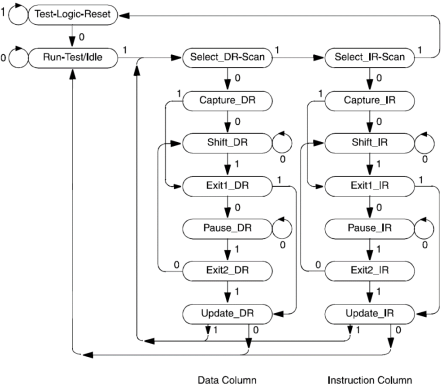
\includegraphics[width=0.5\textwidth]{images/bst_tapkontroller.png}
    \end{figure}
\end{multicols}

\paragraph{Verbindliche Befehle}$~$ \\
Die folgenden Befehle müssen in jedem Fall implementiert sein:
\begin{compactitem}
    \item \textbf{BYPASS}: Der Befehlscode besteht aus lauter Einsen (11...1). Ist dieser Befehl aktiv, muss im Zustand \textit{Shift\_DR} das Bypass-Register in den \textit{TDI}/\textit{TDO} Pfad geschaltet sein. Ebenfalls dürfen die Testregister die Kernlogik nicht beeinflussen.
    \item \textbf{SAMPLE} / \textbf{RELOAD}: Nimmt eine Momentanaufnahme des aktuellen Zustandes der IC-Anschlüsse auf oder setzt die IC-Anschlüsse auf einen definierten Zustand. Das BSR wird im Zustand \textit{Shift\_DR} bei diesem Befehl in den \textit{TDI}/\textit{TDO} Pfad geschalten.
    \item \textbf{EXTEST}: Der Befehlscode besteht aus lauter Nullen (00...0). Die Chiplogik wird bei diesem Befehl von der Leiterplatte isoliert (Die Kernlogik muss so abgeschottet sein, dass sie nicht beschädigt werden kann). Das BSR wird im Zustand \textit{Shift\_DR} bei diesem Befehl in den \textit{TDI}/\textit{TDO} Pfad geschalten.
\end{compactitem}

\paragraph{Interner Aufbau}$~$ \\
Nachfolgend ist dargestellt, wie der TAP-Kontroller intern mit den vorhandenen Registern verschaltet ist.
\begin{figure}[H]
    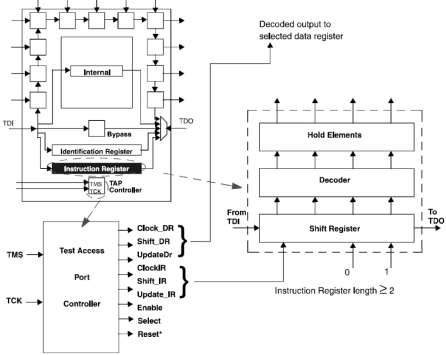
\includegraphics[width=0.75\textwidth]{images/bst_tapkontroller_verschaltung.png}
\end{figure}

\paragraph{Optionale Befehle}$~$ \\
Die nachfolgenden Befehle sind optional, werden jedoch auch häufig implementiert:
\begin{compactitem}
    \item \textbf{INTEST}: Testet die Kernlogik eines Chips. Die Kernlogik wird zu diesem Zweck von den Ein- und Ausgängen isoliert.
    \item \textbf{RUNBIST}: Startet einen eingebauten BIST-Selbsttest. Der Vorteil dieser Variante ist (im Gegensatz zum \textit{INTEST}) dass die Konfiguration des Chips nicht selber vorgenommen werden muss und am Schluss nur das Ergebnis überprüft werden muss.
    \item \textbf{IDCODE}: Liefert den Inhalt aus dem Identifikations-Register zurück.
\end{compactitem}
\begin{multicols}{2}
\subsubsection{Aufbau BYPASS-Register}
\begin{figure}[H]
    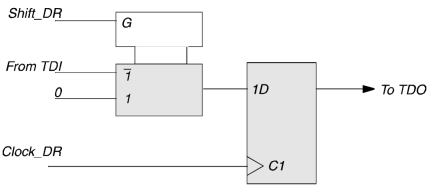
\includegraphics[width=0.5\textwidth]{images/bst_bypassregister.png}
\end{figure}

\subsubsection{Aufbau ID-Register}
Das Identifikations-Register ist immer 32bit breit.
\begin{compactitem}
    \item \textbf{Bit 31-28}: Chip-Version
    \item \textbf{Bit 27-12}: Frei verwendbar vom Hersteller
    \item \textbf{Bit 11-1}: Standardisierter Hersteller Code
    \item \textbf{Bit 0}: Immer 1
\end{compactitem}
\end{multicols}
\subsubsection{Aufbau BSC}
\begin{multicols}{2}
\begin{figure}[H]
    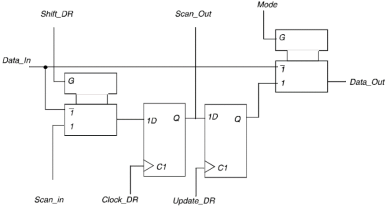
\includegraphics[width=0.5\textwidth]{images/bst_bsc.png}
\end{figure}
Für jeden Ein- und Ausgang eines Chips wird eine Zelle benötigt. Falls aber Three State-Ausgänge oder bidirektionale Anschlüsse vorkommen, dann muss auch deren Enable-Signal mit einer BSC versehen werden. Falls mehrere solcher Signale zu einem Bus zusammengefasst werden, dann werden alle entsprechenden Enable-Signale von derselben BSC geschaltet.
\end{multicols}
